\Scene{3}[Another part of the island.]



\begin{letter}
	\begin{figure}[t!]
		\centering
		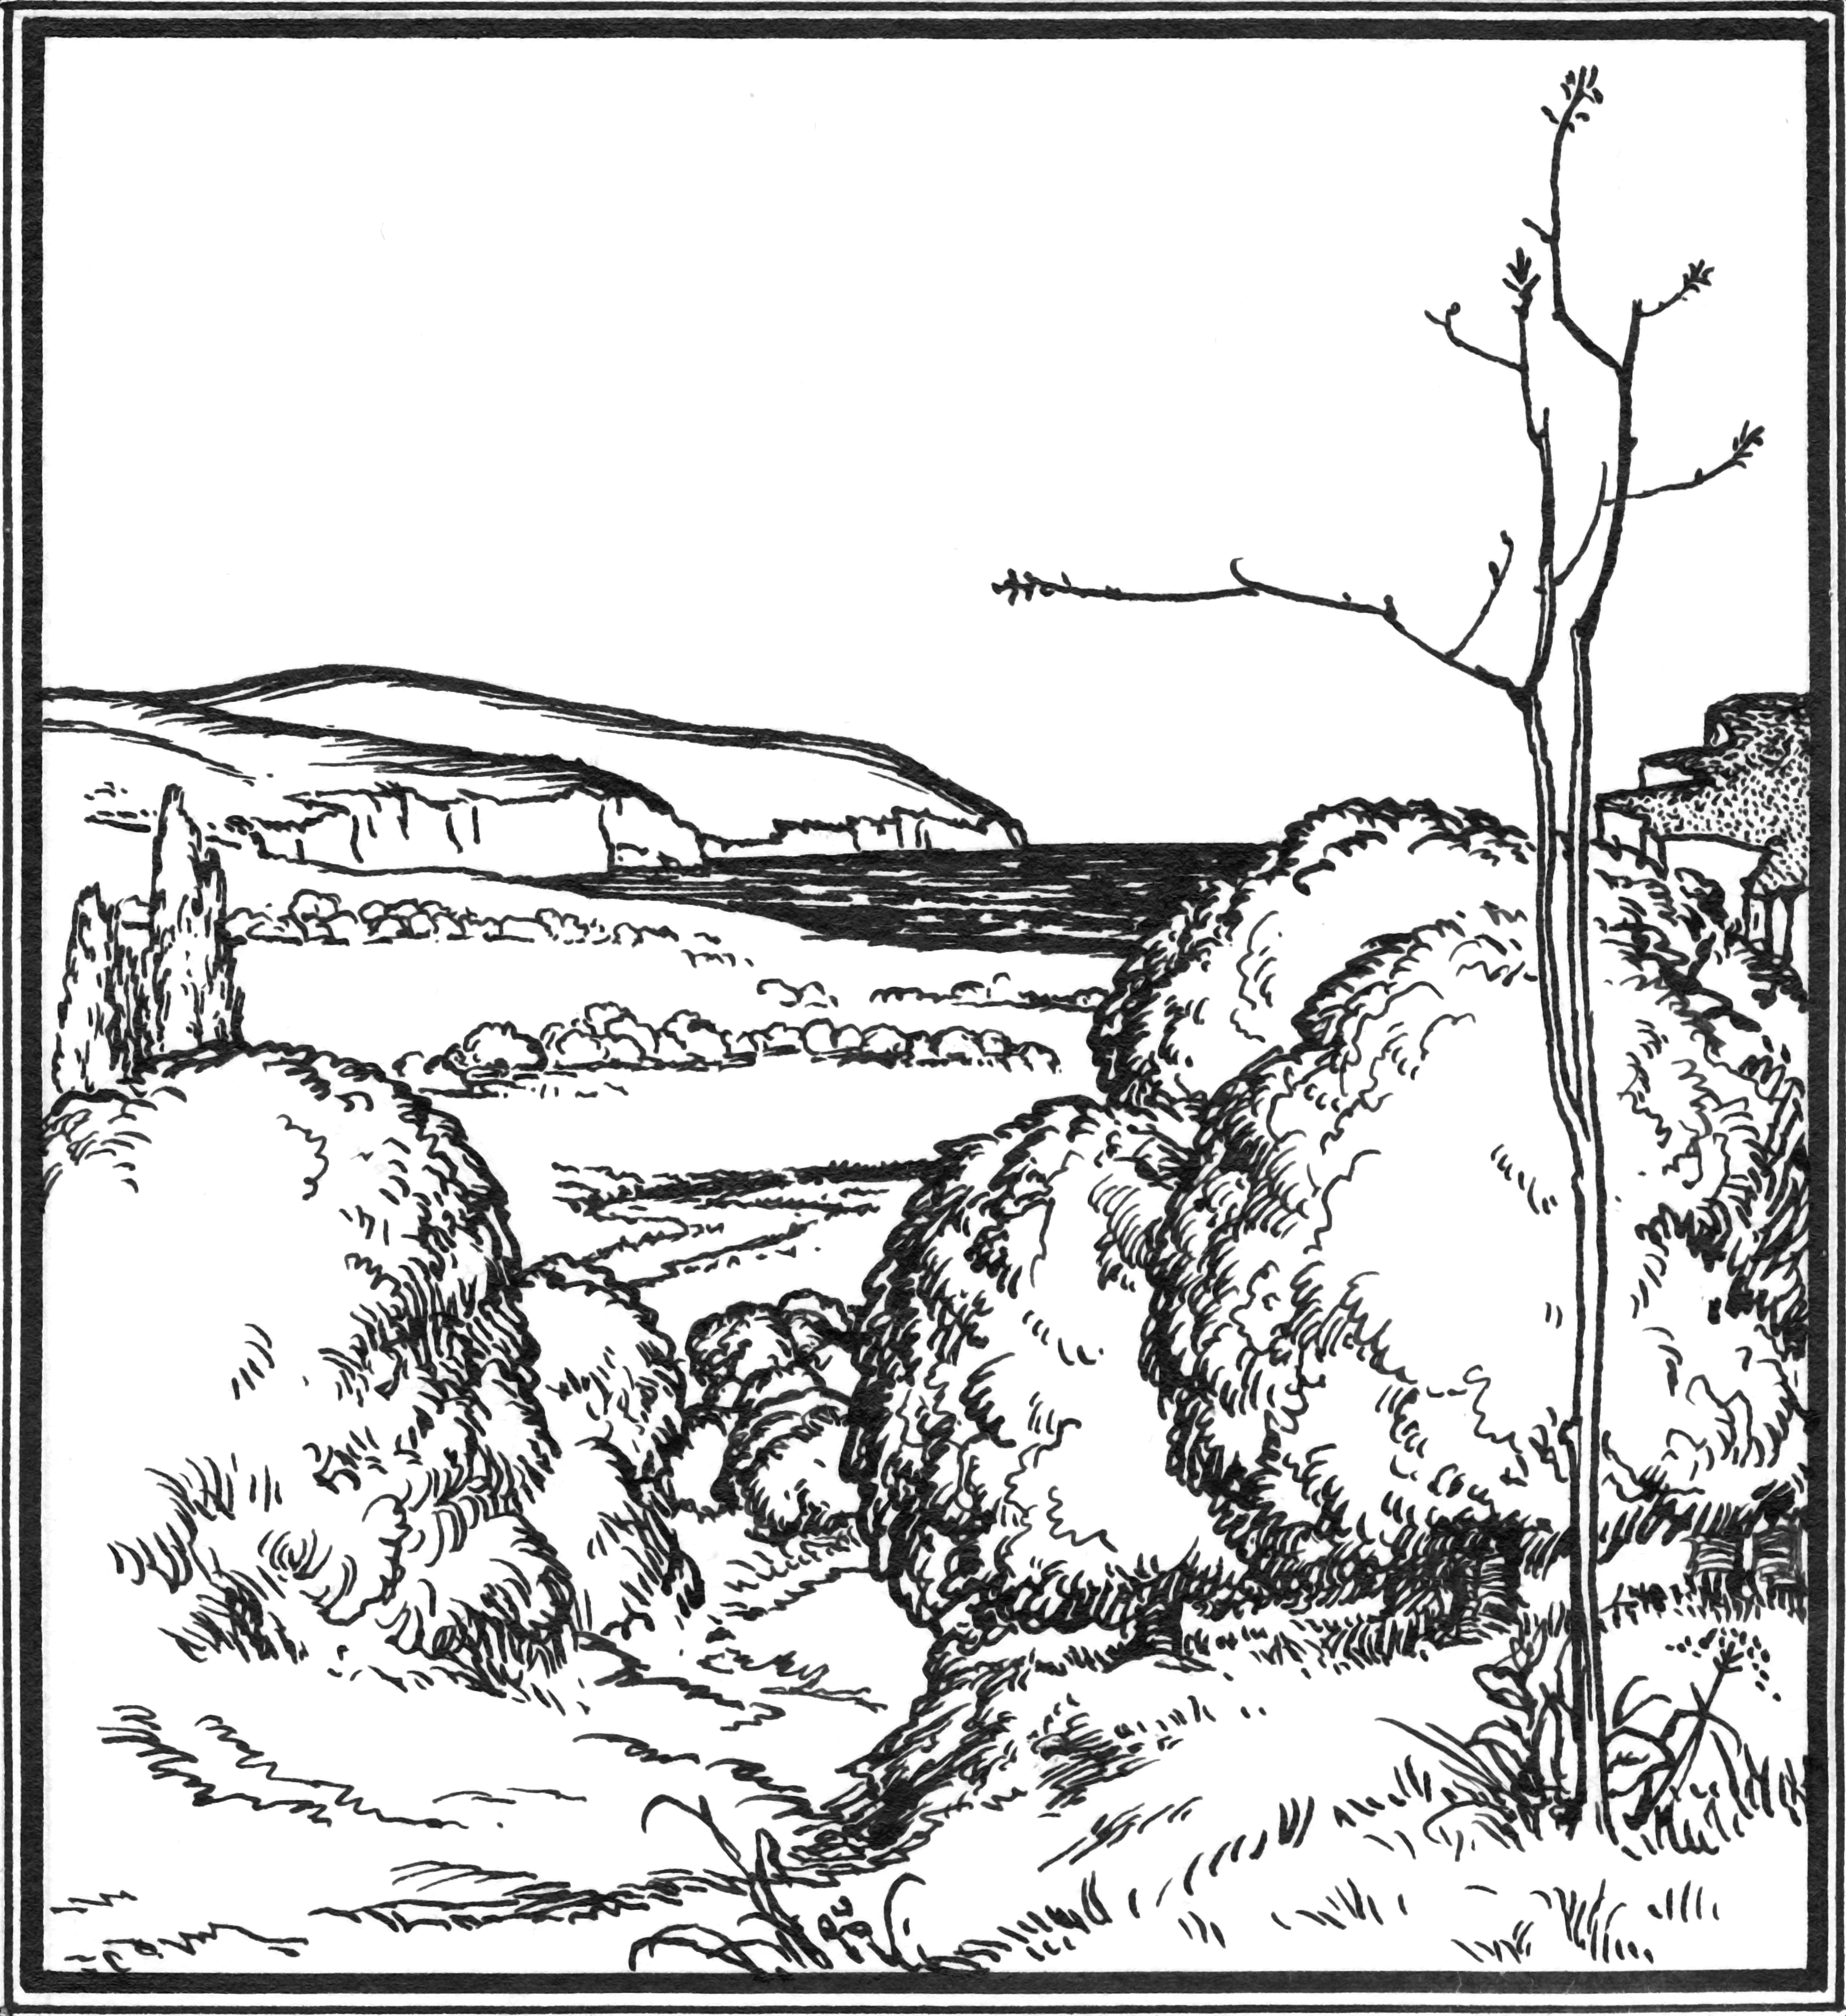
\includegraphics[width=.8\textwidth]{3iiiheadpiece}
	\end{figure}
\end{letter}
\begin{a4}
	\begin{figure}[t!]
		\centering
		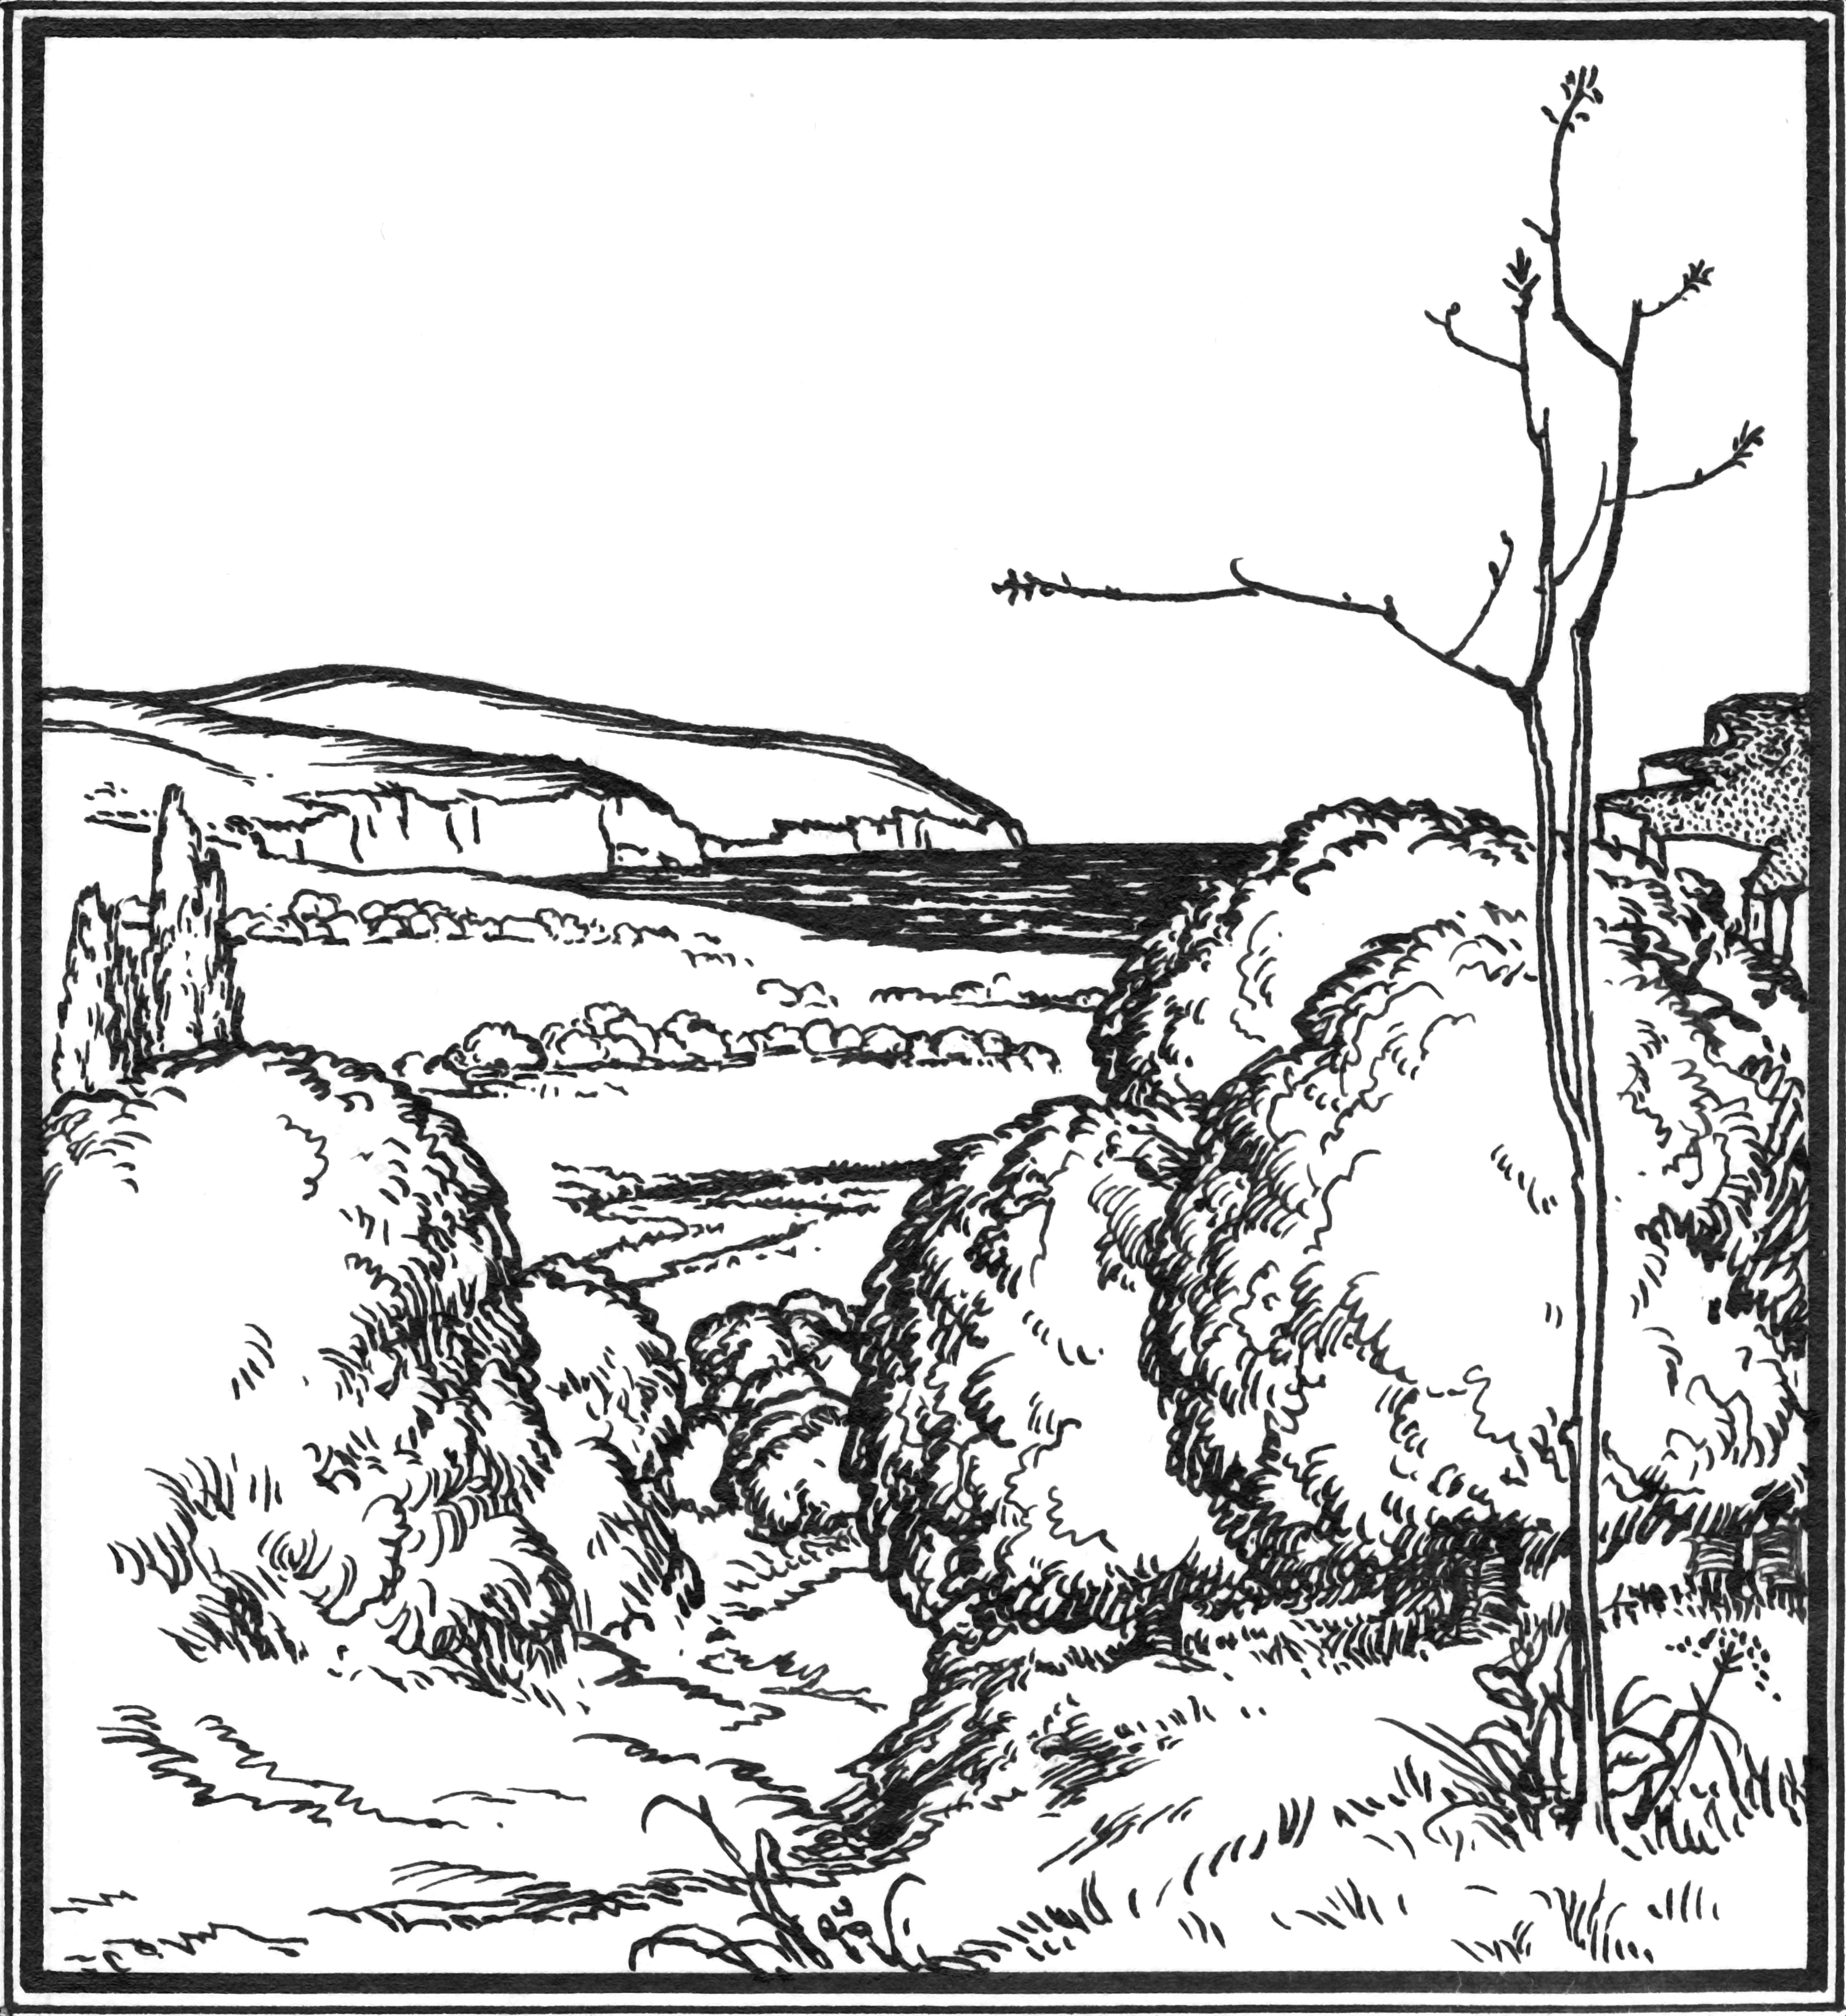
\includegraphics[width=.7\textwidth]{3iiiheadpiece}
	\end{figure}
\end{a4}

\enter{\textsc{Alonso}, \textsc{Sebastian}, \textsc{Antonio}, \textsc{Gonzalo}, \textsc{Adrian}, \textsc{Francisco}, and others}

\begin{letter} %dropcap
	\begin{tikzpicture}[remember picture, overlay]
		\node (dropcap) at ($(current page.west)+(3cm,-6.25cm)$) {
\includegraphics[width=0.125\linewidth]{3iiidropcapB}};
	\end{tikzpicture}
\end{letter}
\begin{a4} 
	\begin{tikzpicture}[remember picture, overlay]
		\node (dropcap) at ($(current page.west)+(3cm,-5.9cm)$) {
\includegraphics[width=0.125\linewidth]{3iiidropcapB}};
	\end{tikzpicture}
\end{a4}

\vspace*{1em}
\begin{verse_speech}[Gonzalo] 
\hspace{2.5em} y'r lakin, I can go no further, sir;\\
My old bones ache: here's a maze trod indeed\\
Through forth-rights and meanders! By your patience,\\
I needs must rest me.
\end{verse_speech}

\begin{verse_speech}[Alonso] 
\hspace{\widthof{I needs must rest me.}}Old lord, I cannot blame thee,\\
Who am myself attach'd with weariness,\\
To the dulling of my spirits: sit down, and rest.\\
Even here I will put off my hope and keep it\\
No longer for my flatterer: he is drown'd\\
Whom thus we stray to find, and the sea mocks\\
Our frustrate search on land. Well, let him go.
\end{verse_speech}

\begin{verse_speech}[Antonio] 
\asideto{Sebastian}{I am right glad that he's so out of hope.\\
Do not, for one repulse, forego the purpose\\
That you resolved to effect.}
\end{verse_speech}

\begin{verse_speech}[Sebastian] 
\asideto{Antonio}{\hspace{\widthof{That you resolved to effect.}-\widthof{[Aside to Antonio]}}The next advantage\\
Will we take throughly.}
\end{verse_speech}

\begin{verse_speech}[Antonio] 
\asideto{Sebastian}{
\hspace{\widthof{Will we take throughly.}-\widthof{[Aside to Sebastian]}}Let it be to-night;\\
For, now they are oppress'd with travel, they\\
Will not, nor cannot, use such vigilance\\
As when they are fresh.}
\end{verse_speech}

\begin{a4}
	\begin{figure}[tb]
		\centering
		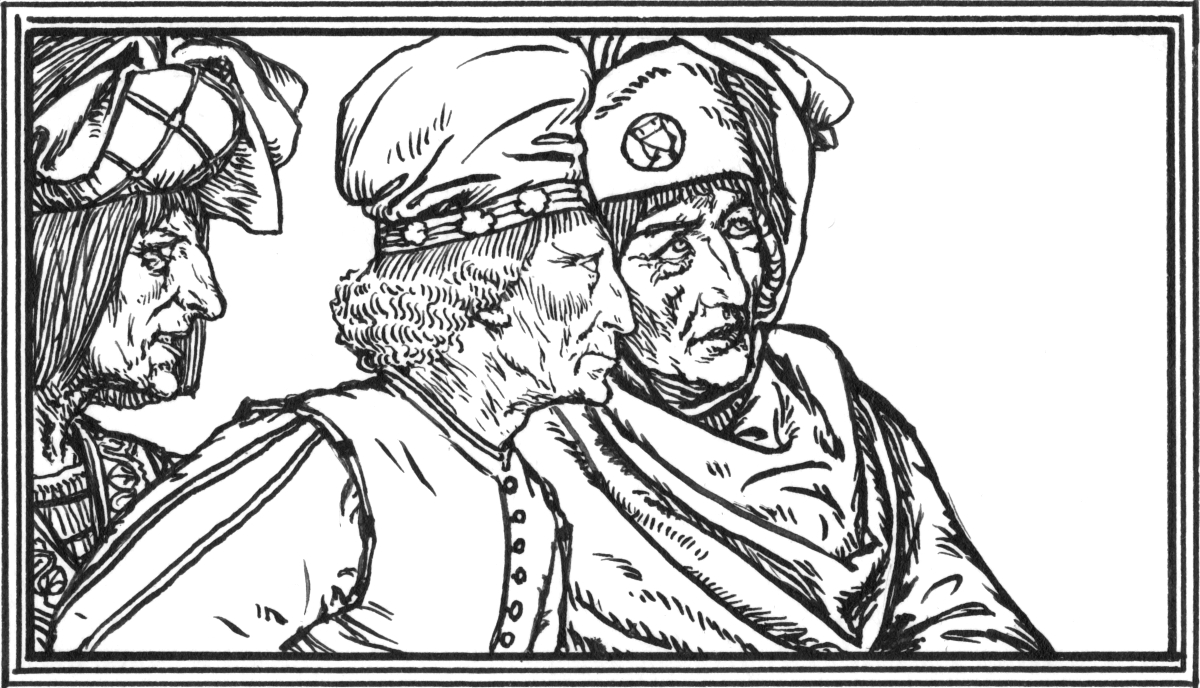
\includegraphics[width=\textwidth]{3iiiconspire}
	\end{figure}
\end{a4}

\verseline[Sebastian]{\asideto{Antonio}{\hspace{\widthof{As when they are fresh.}-\widthof{[Aside to Antonio]}}I say, to-night: no more.}}

\stage{Solemn and strange music}

\verseline[Alonso]{What harmony is this? My good friends, hark!}

\verseline[Gonzalo]{Marvellous sweet music!}



\enter{\textsc{Prospero} above, invisible. Enter several strange Shapes, bringing in a banquet; they dance about it with gentle actions of salutation; and, inviting the King, \&c. to eat, they depart}

\verseline[Alonso]{Give us kind keepers, heavens! What were these?}

\begin{verse_speech}[Sebastian] 
A living drollery. Now I will believe\\
That there are unicorns, that in Arabia\\
There is one tree, the phoenix' throne, one phoenix\\
At this hour reigning there.
\end{verse_speech}

\begin{verse_speech}[Antonio] 
\hspace{\widthof{At this hour reigning there.}}I'll believe both;\\
And what does else want credit, come to me,\\
And I'll be sworn 'tis true: travellers ne'er did lie,\\
Though fools at home condemn 'em.
\end{verse_speech}

\begin{verse_speech}[Gonzalo] 
\hspace{\widthof{Though fools at home condemn 'em.}}If in Naples\\
I should report this now, would they believe me?\\
If I should say, I saw such islanders—\\
For, certes, these are people of the island—\\
Who, though they are of monstrous shape, yet, note,\\
Their manners are more gentle-kind than of\\
Our human generation you shall find\\
Many, nay, almost any.
\end{verse_speech}

\begin{letter}
	\begin{bwbigpic}
		[\picwidth]
		{3iiibanquetleft}
		{}
	\end{bwbigpic}
	\begin{bwbigpic}
		[\picwidth]
		{3iiibanquetright}
		{}
	\end{bwbigpic}
\end{letter}


\begin{verse_speech}[Prospero]
\aside{\hspace{\widthof{Many, nay, almost any.}-\widthof{[Aside]}}Honest lord,\\
Thou hast said well; for some of you there present\\
Are worse than devils.}
\end{verse_speech}


\begin{verse_speech}[Alonso] 
\hspace{\widthof{Are worse than devils.}}I cannot too much muse\\
Such shapes, such gesture and such sound, expressing,\\
Although they want the use of tongue, a kind\\
Of excellent dumb discourse.
\end{verse_speech}

\verseline[Prospero]{\aside{\hspace{\widthof{Of excellent dumb discourse.}-\widthof{[Aside]}}Praise in departing.}}

\verseline[Francisco]{They vanish'd strangely.}

\begin{verse_speech}[Sebastian] 
No matter, since\\
They have left their viands behind; for we have stomachs.\\
Will't please you taste of what is here?
\end{verse_speech}

\begin{a4}
	\begin{bwbigpic}
		[\picwidth]
		{3iiibanquetleft}
		{}
	\end{bwbigpic}
	\begin{bwbigpic}
		[\picwidth]
		{3iiibanquetright}
		{}
	\end{bwbigpic}

\end{a4}

\verseline[Alonso]{\hspace{\widthof{Will't please you taste of what is here?}}Not I.}

\begin{letter}
	\begin{figure}[tb]
		\centering
		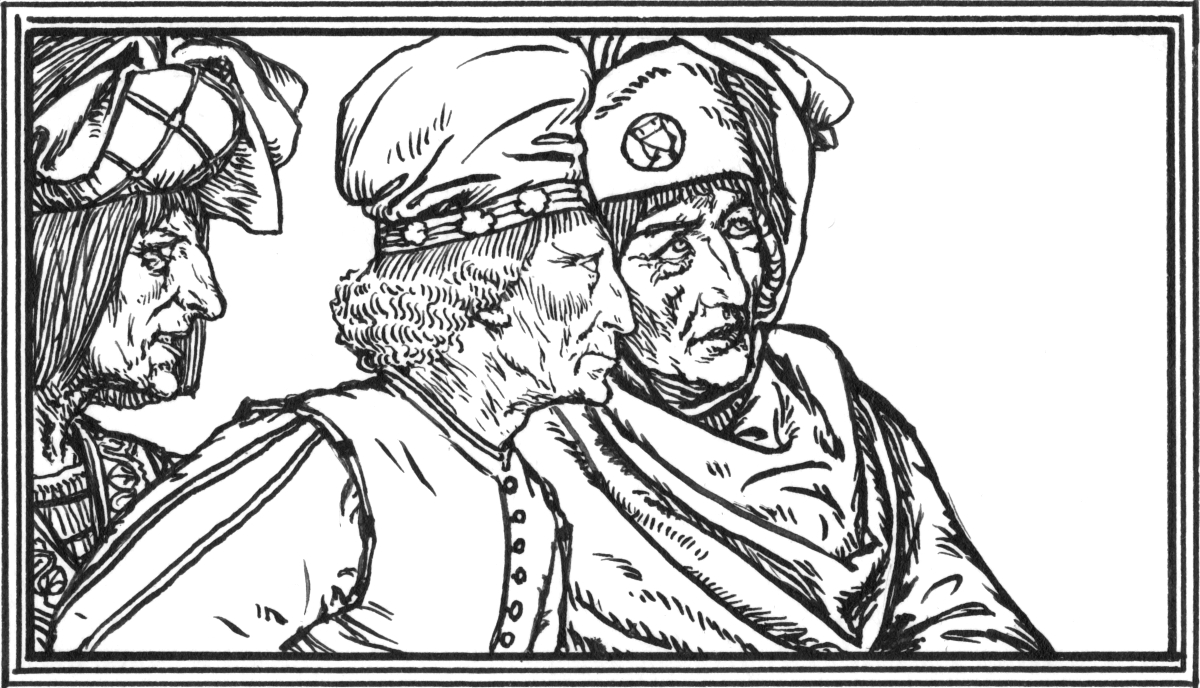
\includegraphics[width=\textwidth]{3iiiconspire}
	\end{figure}
\end{letter}

\begin{verse_speech}[Gonzalo] 
Faith, sir, you need not fear. When we were boys,\\
Who would believe that there were mountaineers\\
Dew-lapp'd like bulls, whose throats had hanging at 'em\\
Wallets of flesh? or that there were such men\\
Whose heads stood in their breasts? which now we find\\
Each putter-out of five for one will bring us\\
Good warrant of.
\end{verse_speech}

\begin{verse_speech}[Alonso] 
\hspace{\widthof{Good warrant of.}}I will stand to and feed,\\
Although my last: no matter, since I feel\\
The best is past. Brother, my lord the duke,\\
Stand to and do as we.
\end{verse_speech}

\begin{letter}
	\begin{figure}[tb]
		\centering
		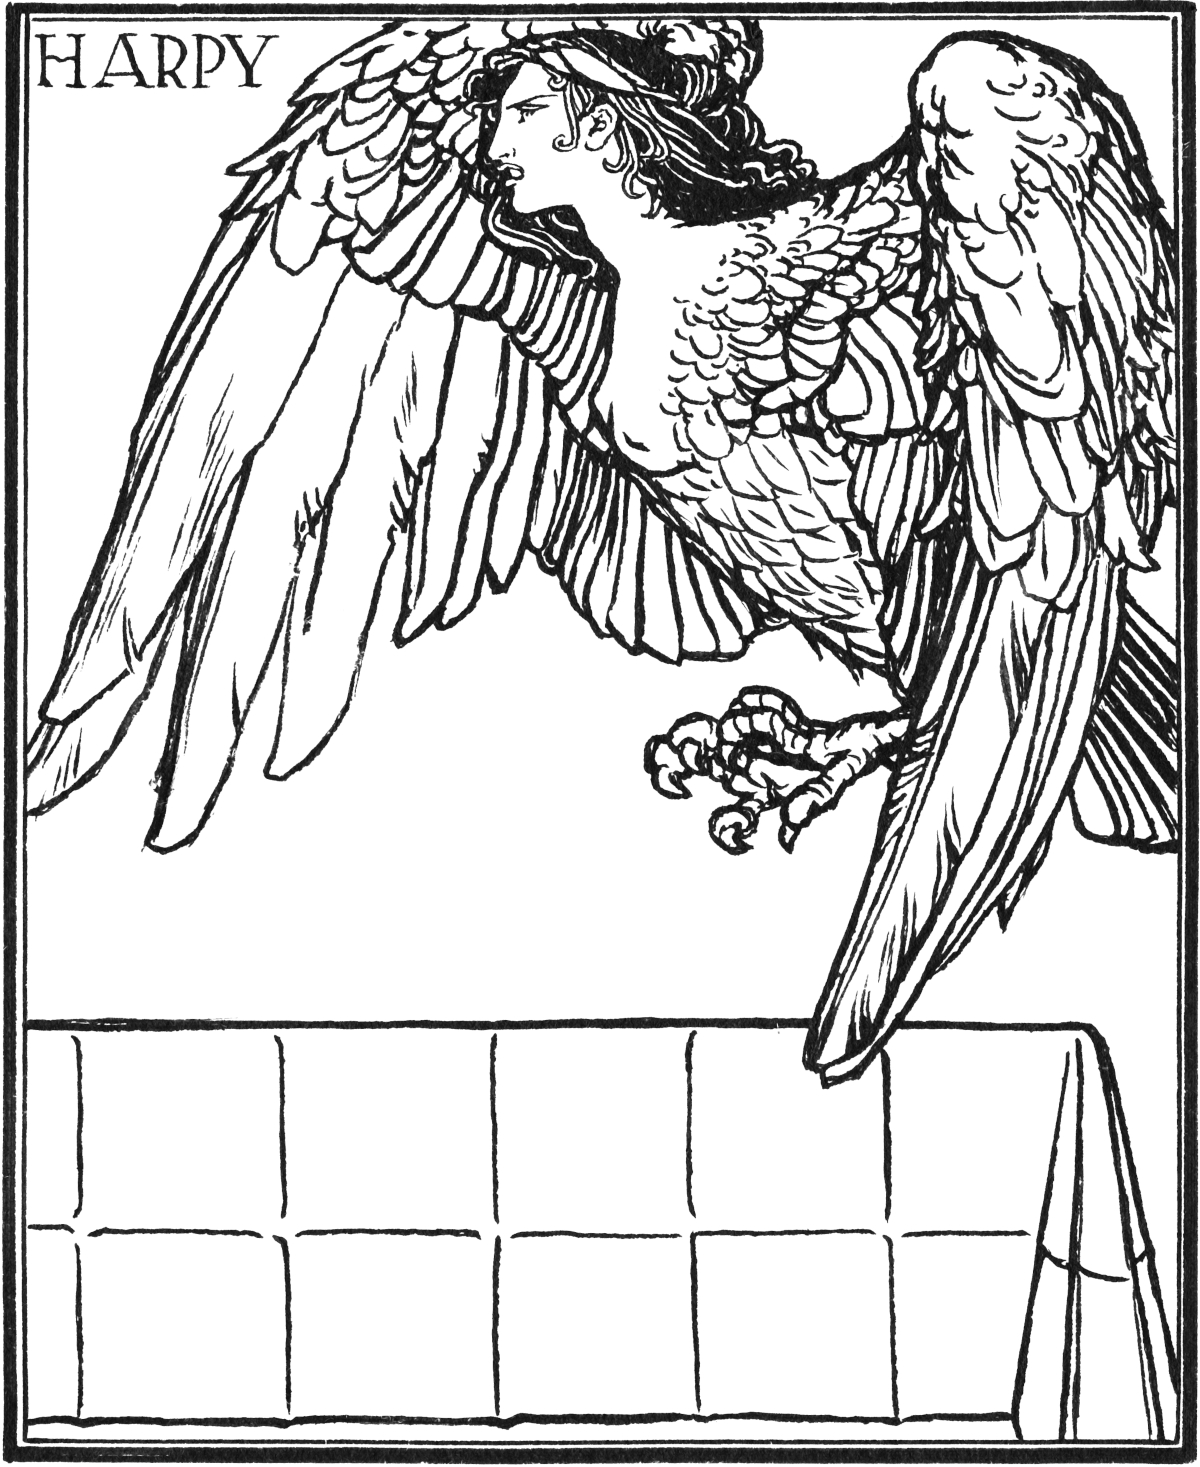
\includegraphics[width=.75\textwidth]{3iiiharpy}
	\end{figure}
\end{letter}
\begin{a4}
	\begin{figure}[tb]
		\centering
		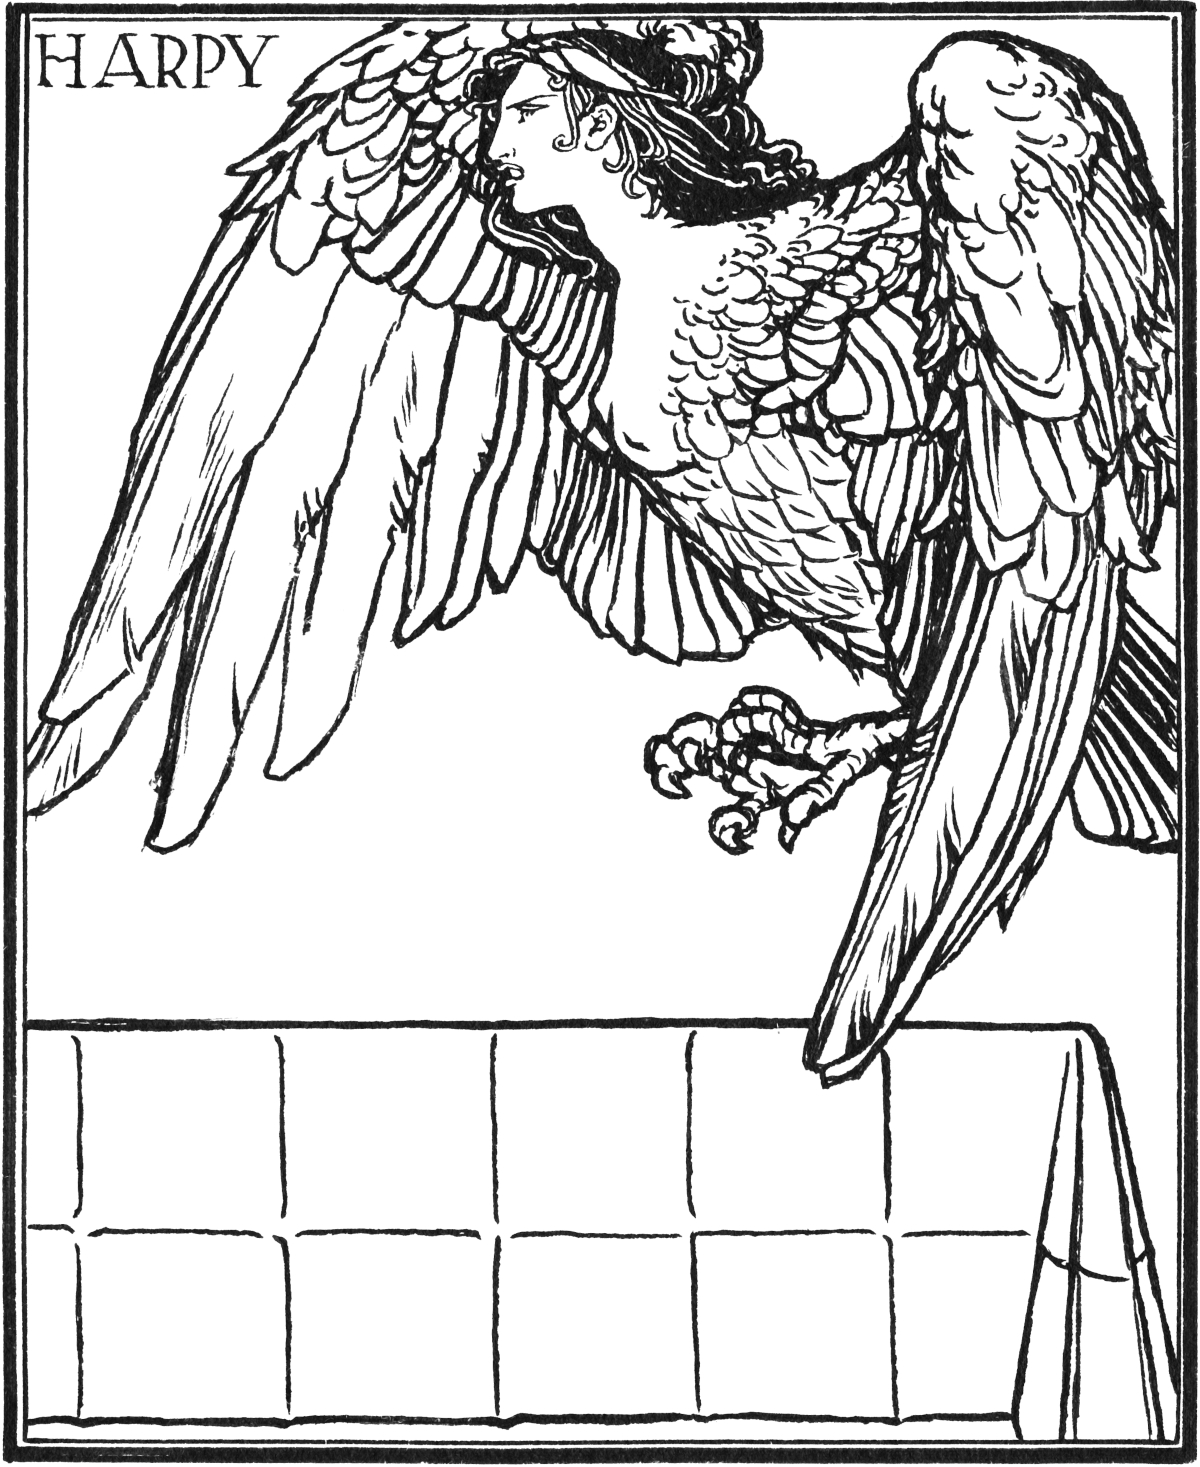
\includegraphics[width=.7\textwidth]{3iiiharpy}
	\end{figure}
\end{a4}

\stage{Thunder and lightning. Enter \textsc{Ariel}, like a harpy; claps his wings upon the table; and, with a quaint device, the banquet vanishes}

\begin{verse_speech}[Ariel] 
You are three men of sin, whom Destiny,\\
That hath to instrument this lower world\\
And what is in't, the never-surfeited sea\\
Hath caused to belch up you; and on this island\\
Where man doth not inhabit; you 'mongst men\\
Being most unfit to live. I have made you mad;\\
And even with such-like valour men hang and drown\\
Their proper selves.

\stage{\textsc{Alonso}, \textsc{Sebastian} \&c. draw their swords}

\hspace{\widthof{Their proper selves.}}You fools! I and my fellows\\
Are ministers of Fate: the elements,\\
Of whom your swords are temper'd, may as well\\
Wound the loud winds, or with bemock'd-at stabs\\
Kill the still-closing waters, as diminish\\
One dowle that's in my plume: my fellow-ministers\\
Are like invulnerable. If you could hurt,\\
Your swords are now too massy for your strengths\\
And will not be uplifted. But remember—\\
For that's my business to you—that you three\\
From Milan did supplant good Prospero;\\
Exposed unto the sea, which hath requit it,\\
Him and his innocent child: for which foul deed\\
The powers, delaying, not forgetting, have\\
Incensed the seas and shores, yea, all the creatures,\\
Against your peace. Thee of thy son, Alonso,\\
They have bereft; and do pronounce by me:\\
Lingering perdition, worse than any death\\
Can be at once, shall step by step attend\\
You and your ways; whose wraths to guard you from—\\
Which here, in this most desolate isle, else falls\\
Upon your heads—is nothing but heart-sorrow\\
And a clear life ensuing.
\end{verse_speech}


\stage{He vanishes in thunder; then, to soft music, enter the Shapes again, and dance, with mocks and mows, and carrying out the table}

\begin{verse_speech}[Prospero] 
Bravely the figure of this harpy hast thou\\
Perform'd, my Ariel; a grace it had, devouring:\\
Of my instruction hast thou nothing bated\\
In what thou hadst to say: so, with good life\\
And observation strange, my meaner ministers\\
Their several kinds have done. My high charms work\\
And these mine enemies are all knit up\\
In their distractions; they now are in my power;\\
And in these fits I leave them, while I visit\\
Young Ferdinand, whom they suppose is drown'd,\\
And his and mine loved darling.
\end{verse_speech}

\stage{He exits, above.}

\begin{verse_speech}[Gonzalo] 
I' the name of something holy, sir, why stand you\\
In this strange stare?
\end{verse_speech}

\begin{verse_speech}[Alonso] 
\hspace{\widthof{In this strange stare?}}O, it is monstrous, monstrous:\\
Methought the billows spoke and told me of it;\\
The winds did sing it to me, and the thunder,\\
That deep and dreadful organ-pipe, pronounced\\
The name of Prosper: it did bass my trespass.\\
Therefore my son i' the ooze is bedded, and\\
I'll seek him deeper than e'er plummet sounded\\
And with him there lie mudded.
\end{verse_speech}

\exit{}

\begin{verse_speech}[Sebastian] 
But one fiend at a time,\\
I'll fight their legions o'er.
\end{verse_speech}

\verseline[Antonio]{\hspace{\widthof{I'll fight their legions o'er.}}I'll be thy second.}

\exit{\textsc{Sebastian} and \textsc{Antonio}}

\begin{verse_speech}[Gonzalo] 
All three of them are desperate: their great guilt,\\
Like poison given to work a great time after,\\
Now 'gins to bite the spirits. I do beseech you\\
That are of suppler joints, follow them swiftly\\
And hinder them from what this ecstasy\\
May now provoke them to.
\end{verse_speech}

\verseline[Adrian]{\hspace{\widthof{May now provoke them to.}}Follow, I pray you.}

\exeunt{}

\begin{center}
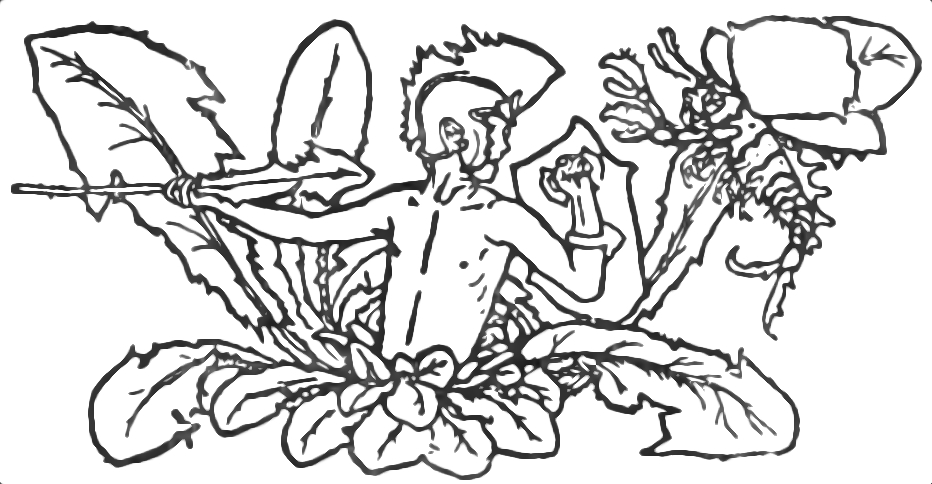
\includegraphics[width=.5\textwidth]{3iiitailpiece}
\end{center}